    % 编译使用xelatex
\documentclass{ctexart}

\usepackage{amsmath}
\usepackage{amsfonts}
\usepackage{amssymb}
\usepackage{graphicx}
\usepackage{subfigure}

\DeclareMathOperator{\Zset}{\mathbb{Z}}

\title{计算机网络安全技术}

\begin{document}
\maketitle

\tableofcontents

\section{基本密码学}
\subsection{基本概念}
\paragraph{传统加密和私钥加密} 传统加密包含代换, 置换密码及其组合, 重点依赖于算法的保密.
    私钥加密亦称非对称加密, 算法和公约公开, 私钥保密.
\paragraph{块加密和流加密} 输入是字符, 每次是处理一个字符还是处理一组字符.
\paragraph{无条件安全和计算安全} 无条件安全即, 拥有无论多少密文对破译都没有帮助.
    计算安全即, 破译代价大于加密数据本身价值, 或者破译时间长于加密数据有效时间.
\paragraph{记号}
    \begin{description}
        \item[加密函数] $c = E_{K_E}(m),\quad m \in \mathcal{M}, c \in \mathcal{C}, K_E \in \mathcal{K}_E$
        \item[解密函数] $m = D_{K_D}(c),\quad c \in \mathcal{C}, m \in \mathcal{M}, K_D \in \mathcal{K}_D$
    \end{description}

\subsection{代换密码}
    如Caesar密码等单表代换密码, Playfair密码和Vigenere密码等多表代换密码.
\paragraph{攻击} 拥有足够密文即可通过统计学分析破译.

\subsection{置换密码}
    $D(m) = \sigma m$, 要求$\mathcal{M} = \Sigma^L$, $\sigma$是$[0, L)$上的置换.
\paragraph{攻击} 频率分析, 包括多元组频率分析.

%   *** 不写S-DES了 ***
%\subsection{DES算法}
%    对称加密, $K_D = K_E$, 密钥通过秘密信道分配. 课程介绍DES的一个简化版本S-DES.
%    是一个块加密算法, 输入输出是8位的, 密钥是10位的.
%    分为两步: 计算次密钥$K_1$, $K_2$, 之后利用次密钥加密.\par
%    具体过程略.
%\paragraph{次密钥加密}
%    有如下元素 \begin{enumerate}
%        \item 文字$M = \langle M_0, \ldots M_9 \rangle$
%        \item 密钥$K = \langle K_0, \ldots K_9 \rangle$
%        \item $\sigma_i$是已知的8位置换
%        \item $\sigma_{SW}$是已知的8位置换
%        \item $f_{K_i}$是8位到8位的函数, 由次密钥$K_i$参数化
%        \item $\sigma{LS, l}$是一个已知的10位置换
%    \end{enumerate}
%    则有 \begin{align*}
%        D(M) &= \sigma_i^{-1} ( f_{K_2} ( \sigma_{SW} ( f_{K_1} ( \sigma_i (M) ) ) ) ) \\
%        E(C) &= \sigma_i^{-1} ( f_{K_1} ( \sigma_{SW} ( f_{K_2} ( \sigma_i (C) ) ) ) )
%    \end{align*}
%    其中$f_{K_i}(X)$的定义如下.\par
%    有如下元素 \begin{enumerate}
%        \item $EP$是已知的4位到8位的函数
%        \item $S0, S1$是已知的4位到2位的函数
%        \item $\sigma_4$是4位置换
%    \end{enumerate}
%    则算法如下 (以下特别使用大段顺序) \begin{enumerate}
%        \item $t = EP(X_{3 \ldots 0}) \oplus K_i$
%        \item $h = X_{7 \ldots 4} \oplus \sigma_4(S0(t_{7 \ldots 4}) , S1(t_{3 \ldots 0}))$
%        \item $f_{K_i}(X) = (h, X_{3 \ldots 0})$
%    \end{enumerate}
%\paragraph{计算$K_1, K_2$}
%    有如下元素 \begin{enumerate}
%    \end{enumerate}

\subsection{Feistel密码结构}
\paragraph{Feistel的密码观点}
    \begin{enumerate}
        \item 使用乘积密码
        \item 交替使用代换和置换
    \end{enumerate}
\paragraph{Shannon的密码观点}
    \begin{description}
        \item[扩散] 密文不包含明文的统计信息, 每个明文字符影响多个密文字符
        \item[混淆] 复杂的密文和密钥间的统计关系, 防止从密文推出密钥
    \end{description}
\paragraph{Feistel网络}
    大致如图所示.
    \begin{figure*}[ht]
    \vskip 0.2in
    \begin{center}
    \centerline{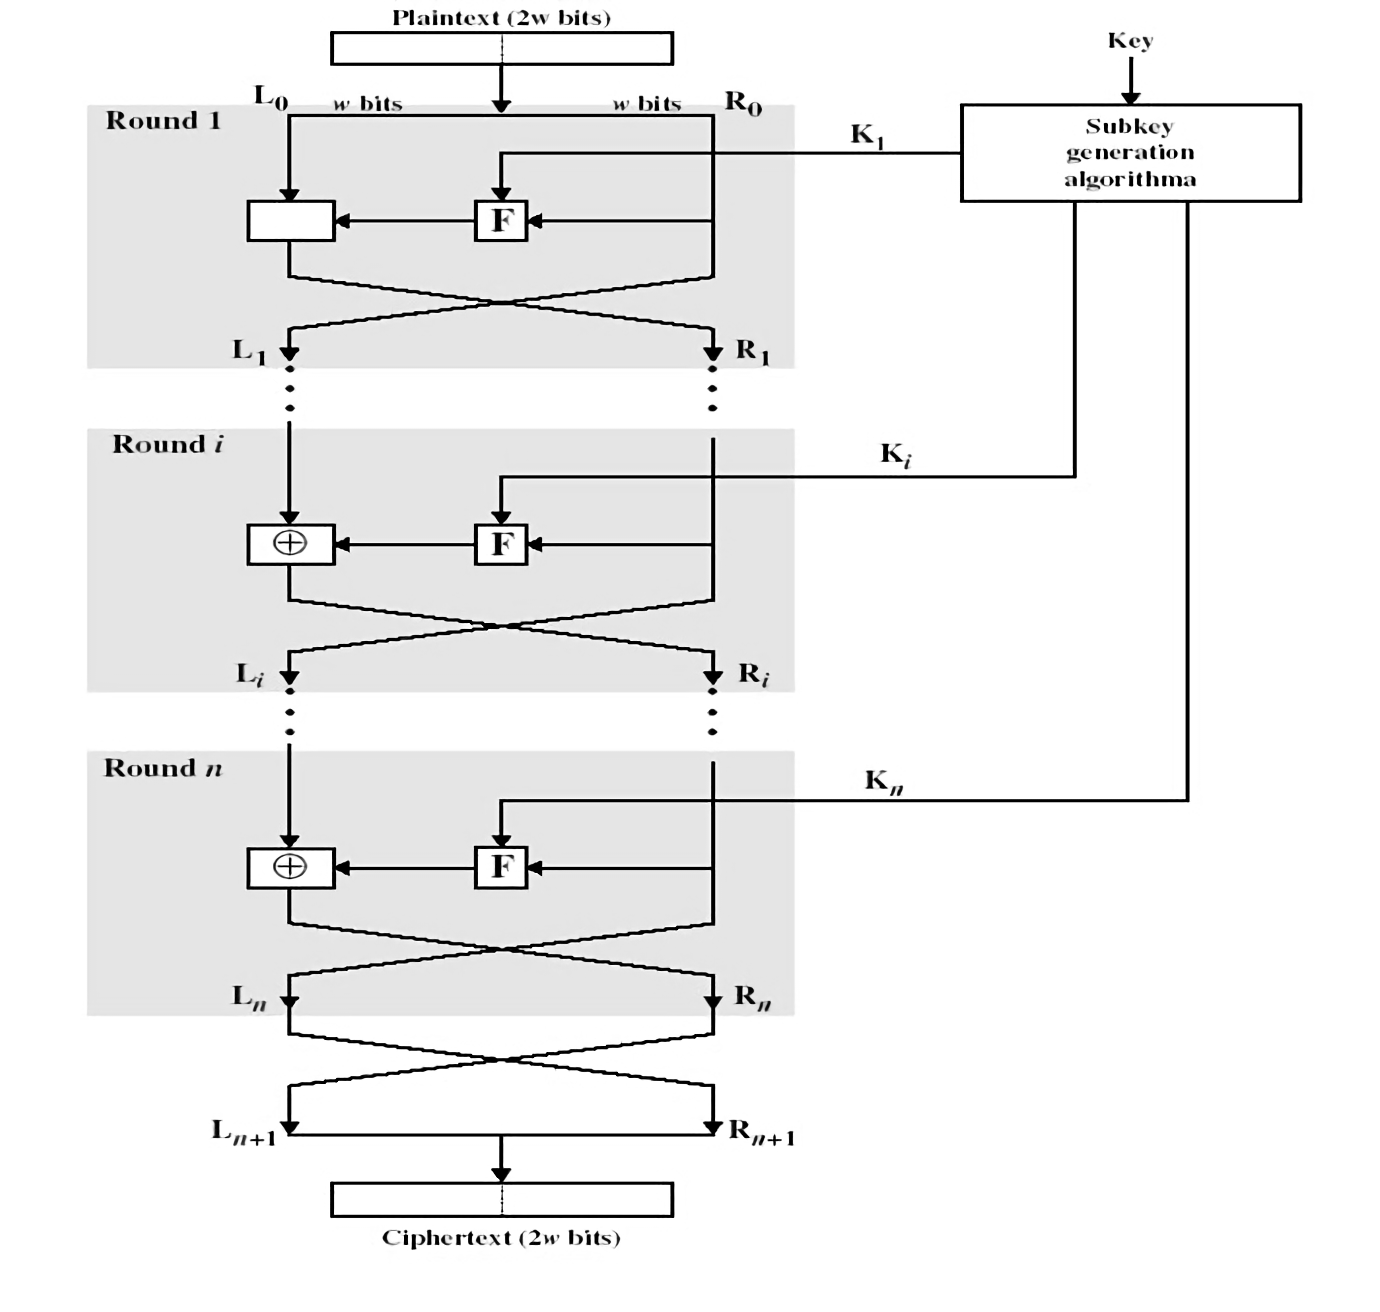
\includegraphics[width=0.6\textwidth]{feistel-net}}
    \caption{经典的Feistel网络结构}
    \label{lenet-structure}
    \end{center}
    \vskip -0.2in
    \end{figure*}
\paragraph{Feistel网络的元素}
    \begin{description}
        \item[分组长度和密钥长度] 越长越安全, 但是效率越低
        \item[迭代层数] 越多越安全
        \item[$K_i$的产生算法] 越复杂越安全
        \item[$F$函数] 越复杂越安全
    \end{description}

\subsection{常见对称密码}
\paragraph{DES算法}
    DES是对称密钥算法, 基于Feistel网络结构.
    密钥长度为56位, 块长度是64位, 迭代16轮.\par
    和Feistel的区别是, 加密初始和末尾有一个置换.\par
    已被破解.
\paragraph{3-DES算法}
    密钥长度加倍到112位, 并且加密函数变成了 \[
        \mathbf{3-DES}(M) = \mathbf{DES}(\mathbf{DES}(\mathbf{DES}(M))) \]
    很安全, 但是效率很低.
\paragraph{Blowfish算法}
    基于Feistel网络结构, 但是每轮中左右两半都进行计算.\par
    未被破解.
\paragraph{RC5算法}
    仍然是多轮加密, 但是每轮结构更加复杂.
\paragraph{AES算法}
    AES不是Feistel结构, 每一轮处理整个输入 (而非分成2部分).

\subsection{RSA算法}
    一种块加密方法, 原文和密文都是$[0, N)$中的整数, 常常$N$是2的幂.\par
\subsubsection{算法}
\paragraph{前置}
    \begin{enumerate}
        \item 计算大素数 $p$, $q$.
        \item 计算$N = pq$, 公开.
        \item 寻找一个小整数$e,\;e < N,\,(e, N) = 1$
        \item 求解$d e \equiv 1 \pmod{\varphi(N) = (p-1)(q-1)}$, 得到$d$
        \item 公钥为$\langle e, N \rangle$, 私钥为$\langle d, N \rangle$
    \end{enumerate}
\paragraph{加密}
    对于$m \in [0, N)$, 加密函数如下
    \[ E(t) = m^e \bmod N \]
\paragraph{解密}
    对于$c \in [0, N)$, 加密函数如下
    \[ D(c) = c^d \bmod N \]
\paragraph{原理}
    有效性由Euler定理保证 \[ a^{\varphi(n)} \equiv 1 \pmod{n},\quad \forall a\,:\,(a, n) = 1 \]
    安全性由大数分解困难性保证.

\subsubsection{攻击}
    \begin{description}
        \item[暴力破解] 需要枚举$t \in [0, N)$的空间
        \item[数学攻击] 因子分解$N$
        \item[计时攻击] 按照加密时间推测私钥.
    \end{description}

\subsection{Diffie-Hellman算法}
    用于密钥交换, 而非加密解密, 即通过双方自身的私有密文得到一个共有密文.
\subsubsection{算法}
\paragraph{前置}
    \begin{enumerate}
        \item 寻找素数$p$, 以及$\Zset_p$的生成元$p$ i.e. $p$是原根, 均公开.
    \end{enumerate}
\paragraph{私有密文产生共有密文}
    \begin{enumerate}
        \item 双方由自己的私有密文$X_A,\, X_B$计算公开的$Y_A = a^{X_A} \bmod p,\, Y_B = a^{X_B} \bmod p$
        \item 双方由公开的$Y_A, Y_B$计算得到共有密文$K = Y_B^{X_A} \bmod p = Y_A^{X_B} \bmod p = a^{X_A X_B} \bmod p$
    \end{enumerate}
\paragraph{原理}
    安全性由离散对数困难性保证.

\subsection{密钥分配}
\subsubsection{传统对称密钥分配}
\paragraph{可能的方法}
    \begin{enumerate}
        \item Alice选择密钥, 亲自交给Bob
        \item 第三方Charlie选择密钥, 亲自交给Alice和Bob
        \item Alice选择密钥, 用最近使用的密钥加密后发给Bob
        \item 第三方Charlie选择密钥, 通过某个秘密渠道交给Alice和Bob
    \end{enumerate}
\paragraph{密钥分发中心}
    基本假设: 每个人有一个仅他自己和KDC知道的主密钥. 此假设下, Alice和Bob得到一次性次密钥的方法为:
    \begin{enumerate}
        \item Alice向KDC请求次密钥
        \item KDC发送给Alice消息, 消息用$PK_a$加密, 包含用次密钥$K_s$, 以及$PK_b$加密的$K_s$和$ID_a$
        \item Alice将$PK_b$加密的消息发送给Bob
    \end{enumerate}
    为了效率和安全性, KDC通常也是层次性的, 而非一个巨大的中心KDC.
\subsubsection{非对称公钥发布}
\paragraph{公开发布} Alice向所有人广播自己的公钥. 问题是容易伪造广播消息.
\paragraph{公开目录} 只有一个受信任的实体 (管理员) 能够广播公钥. 问题是如果受信任的实体被攻击, 公钥可以任意更改.
\paragraph{公钥授权} 双方通讯之前先向管理员请求对方公钥, 管理员返回消息时用管理员私钥加密.
\subsubsection{通过非对称公钥分配传统密钥}
    非对称加密的问题是效率太低, 一般通过非对称加密传输传统密钥, 之后消息用传统加密方法求解.
\paragraph{Merkel朴素方法} Alice给Bob请求共有密钥. Bob用Alice公钥加密某密文后传输给Alice, Alice之后使用自己的私钥解密得到共有密文.
    问题: 中间人攻击, 考虑若Bob是假Bob.
\paragraph{保密真实方法} \begin{enumerate}
        \item Alice发送给Bob: $E_{K_{B, pub}}(ID_A, N_A)$, $N_A$是一个随机校验数
        \item Bob得到$ID_A, N_A$, 发送给Alice: $E_{K_{A, pub}}(N_A, N_B)$
        \item Alice得到$N_A', N_B$, 检查$N_A = N_A'$, 发送给B$E_{K_{B, pub}}(N_B)$
        \item Bob得到$N_B'$, 检查$N_B = n_B'$
    \end{enumerate}


\section{计算机网络安全体系结构}
\subsection{安全目标}
    \begin{description}
        \item[保密性] 未授权的实体不能获得信息内容
        \item[完整性] 信息不能被篡改, 或者能检测篡改
        \item[可用性] 授权用户能够访问资源, 防止DoS攻击
    \end{description}

\section{消息认证}
\subsection{攻击类型}
    \begin{description}
        \item[泄密] 保密性范畴.
        \item[传输分析] 保密性范畴.
        \item[伪装] 消息认证.
        \item[内容修改] 消息认证.
        \item[抵赖] 数字签名, 以及协议设计.
    \end{description}
\subsection{消息认证基本概念}
\subsubsection{消息认证} 确认发送方是真实的, 确认消息违背篡改.
\subsubsection{基本框架} 发送方产生一个认证符; 接收方产生一个认证符, 并且检查双方认证符是否匹配.

\subsection{产生认证符}
\subsubsection{消息加密作为认证符} 对称加密中可以采用这种方式, 但是不能验证消息是否来自正确的发送方.
    解决办法是, 附带原文 (而不是密文) 的校验符号.
    在非对称加密中, 私钥加密只能认证不能加密, 公钥加密则不能认证.
    解决方法是, 接收方公钥发送方私钥两次加密.
\subsubsection{消息认证码MAC}
    通过消息和密钥, 利用公开的算法计算认证 $= C_K(M)$, $K$是共有密钥, $M$是消息.\par
    不能完成数字签名: 接收方也有$K$, 因此可以伪造消息.\par
    实践将一般先加密, 再使用MAC.
\subsubsection{消息的哈希}
    通过消息, 利用公开的算法计算认证符$= \mathbf{Hash}(M)$, $M$是消息. 亦称消息摘要. 
    不同情境下, 其可以提供不同效果, 如\begin{enumerate}
        \item 对称加密中, 可以加密消息和哈希码, 可以完成加密和认证.
        \item 对称加密中, 可以只加密哈希码, 可以完成认证.
        \item 非对称加密中, 用发送方的私钥加密哈希码, 可以完成认证和数字签名.
        \item 非对称加密中, 用发送方的私钥加密消息和哈希码, 可以完成加密, 认证和数字签名.
    \end{enumerate}
\subsection{哈希函数}
\subsubsection{哈希函数的理论要求}
    要求哈希函数$h = H(M)$有如下性质 \begin{description}
        \item[单向性] 对于$h$, 难以寻找$M$, 满足$H(M) = h$
        \item[弱抗碰撞] 对于$M$, 难以寻找$M'$, 满足$H(M) = H(M')$
        \item[强抗碰撞] $\forall M$, 难以寻找$M'$, 满足$H(M) = H(M')$
    \end{description}
\subsubsection{安全哈希函数的Merkel结构} 
    参见图 \ref{merkel-hash}.
    \begin{figure*}[ht]
    \vskip 0.2in
    \begin{center}
    \centerline{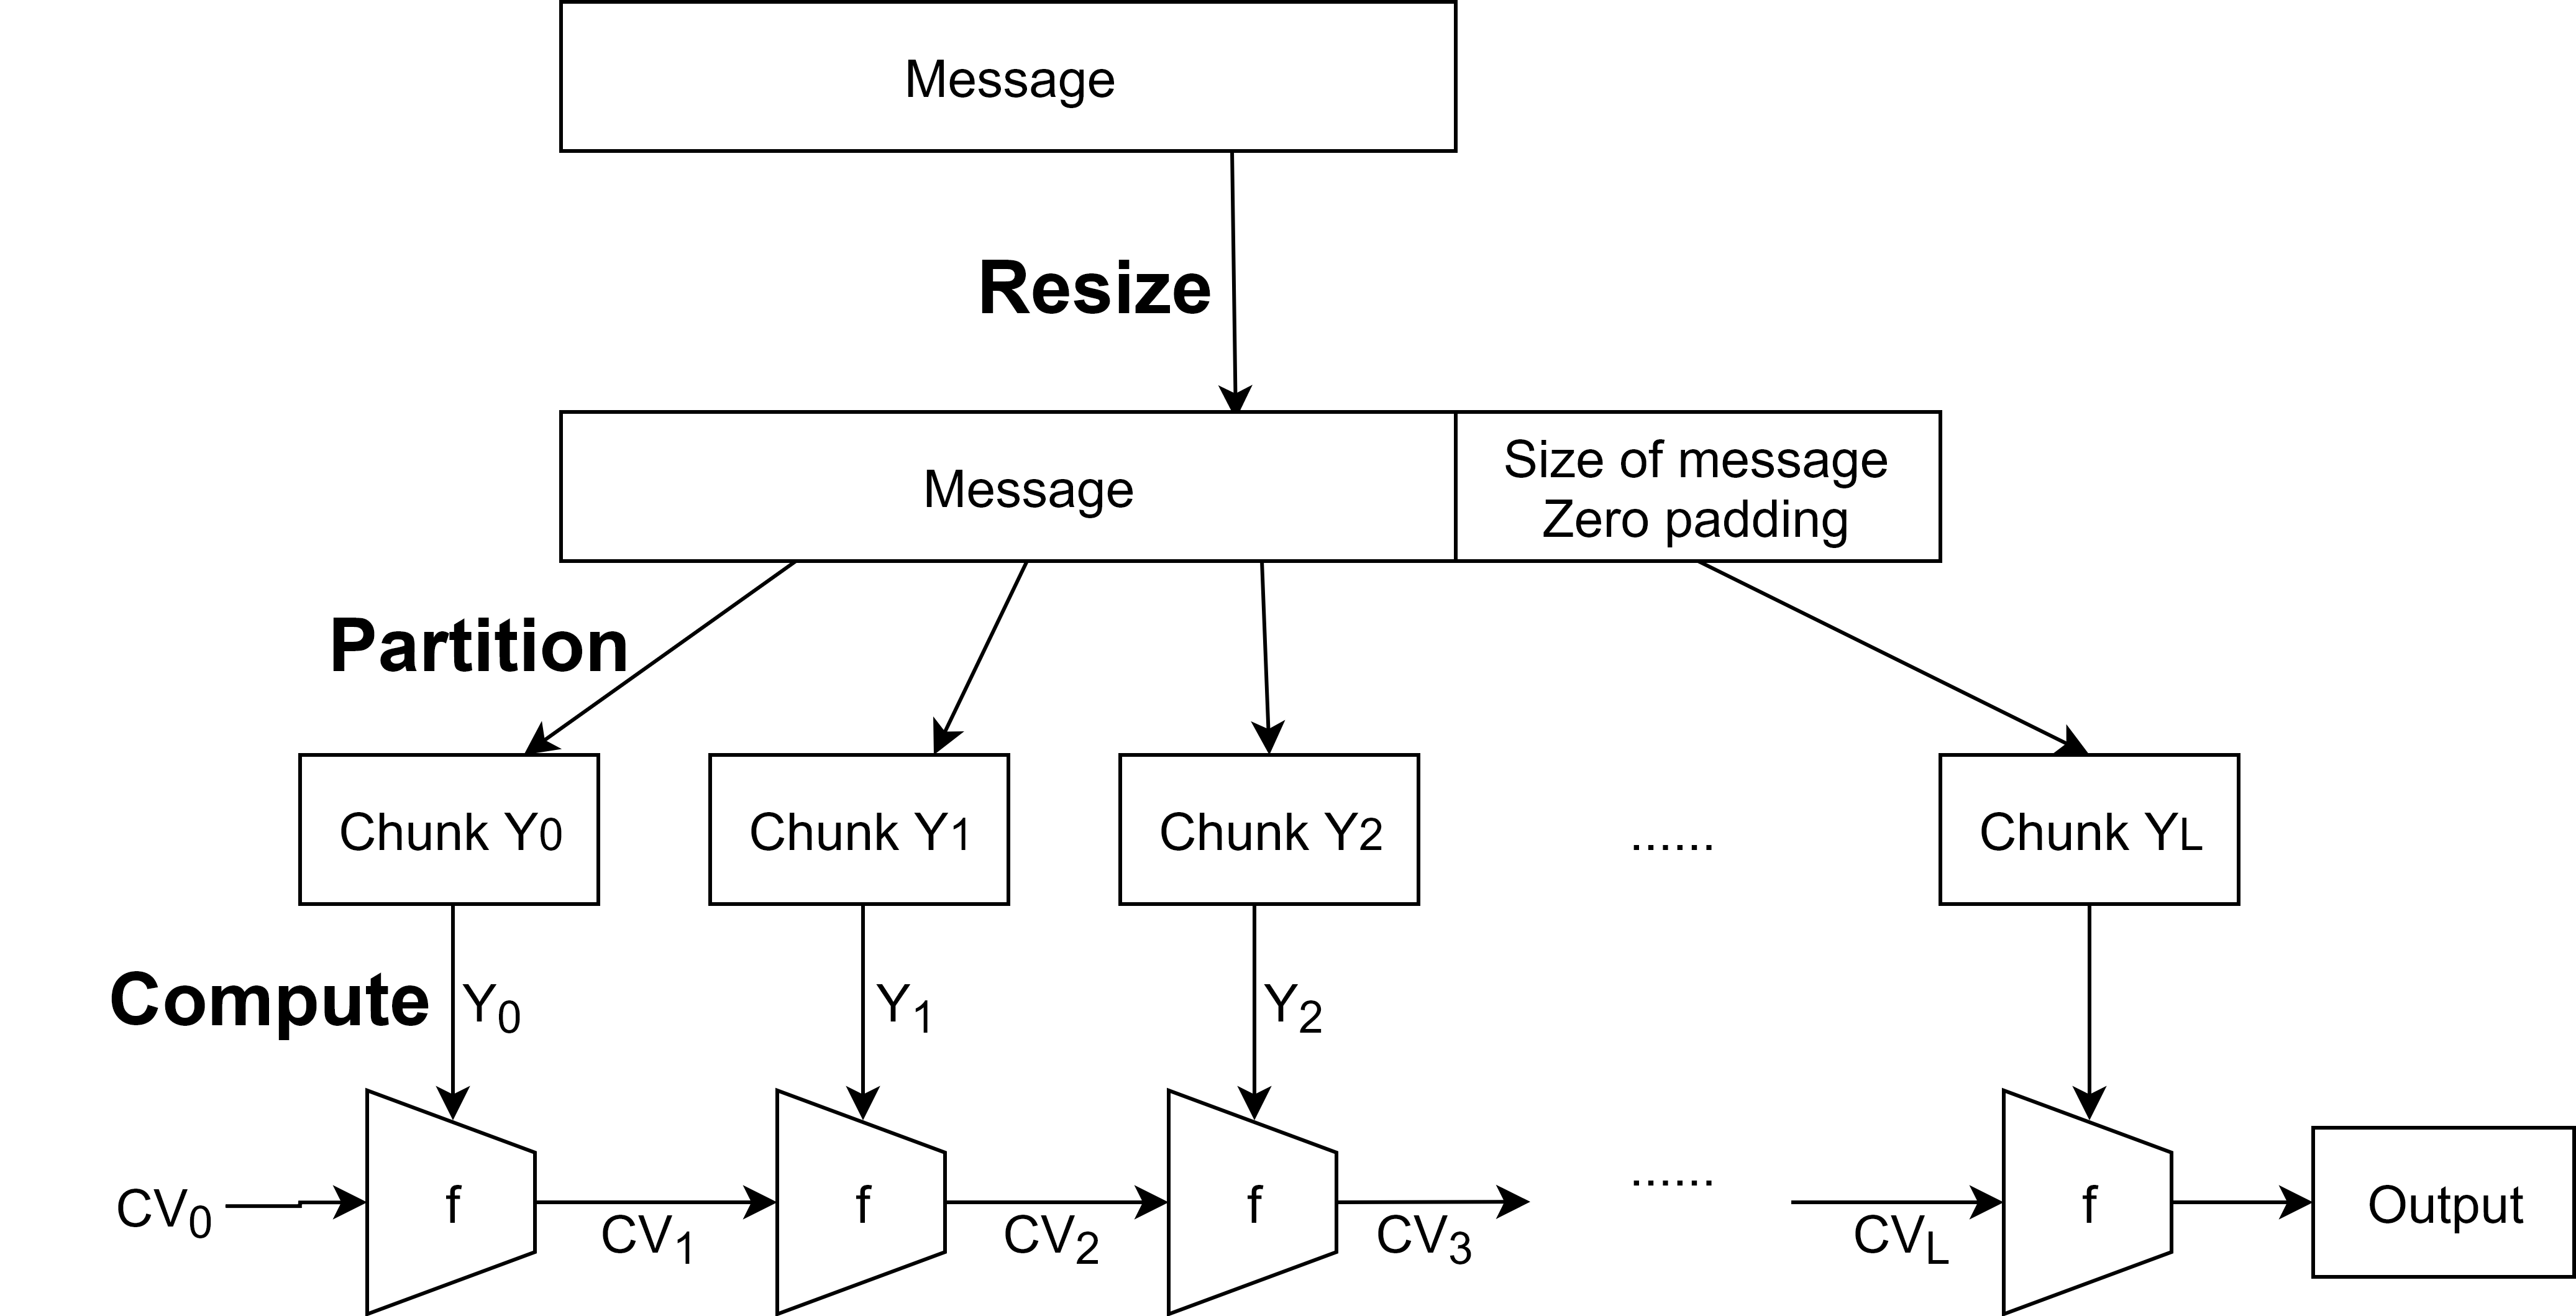
\includegraphics[width=0.8\textwidth]{merkel-hash}}
    \caption{Merkel哈希结构}
    \label{merkel-hash}
    \end{center}
    \vskip -0.2in
    \end{figure*}
\subsubsection{常用哈希举例}  MD5, SHA-1, SHA-2等

\subsection{数字签名DSS算法}
\paragraph{应用场景} 来自消息发送双方的攻击, 如接收方伪造发送, 发送方抵赖发送.
\paragraph{分类} 直接数字签名 (仅通信双方), 仲裁数字签名 (受信任的实体).
\paragraph{前置} \begin{description}
    \item[全局公钥] $p$是素数\\ $q$是素数且$q \mid p -1$\\
        $g = h^{(p-1) / q} \bmod p$
    \item[用户私钥] $x$, 满足$x < q-1$
    \item[用户公钥] $y = g^x \bmod p$
    \item[随机数] $k < q$, 每次认证都应产生一个新的$k$, 且$k$保密
    \end{description}
\paragraph{DSS算法签名} 签名用一组数$(r, s)$代表, 计算过程如下方程, 哈希函数$\mathbf{H}$一般取SHA-1
    \begin{align*}
        r &= g^k \bmod p \bmod q\\
        s &= (k^{-1} (\mathbf{H}(M) + xr)) \bmod q
    \end{align*}验证要求 \begin{equation*}
        g^{(s^{-1} M) \bmod q} y^{(s^{-1} r) \bmod q} = r
    \end{equation*}

\section{访问控制}
\subsection{基本概念}
\paragraph{主体} 提出访问资源请求的人/实体.
\paragraph{客体} 含有被访问资源的实体.
\paragraph{访问} 对资源的使用行为, 有时还需包括主客体.
\paragraph{访问控制矩阵} 定义不同主体对于不同客体可以执行的操作, 如 \[ \begin{array}{|c|c|c|}
        \hline
        & \multicolumn{2}{c}{1} \\ 
        \hline
        3 & 4 & 5 \\
        \hline
    \end{array} \]

\paragraph{3A机制}  认证, 授权, 审计

\subsection{访问控制模型}
\subsubsection{自主性访问控制} 每个客体有一个管理者, 管理者将访问权限授权给其他人. 可以看成以主体为核心.
\paragraph{性质} 易用方便灵活. 但是不能控制信息的流动, i.e. 其他人取得资源后可以自由分发.
\subsubsection{强制性访问控制} 每个主体和客体有固定的安全级别, 由系统管理员决定. 可以看成以客体为核心.
\paragraph{No Read Up} 主体只能读取安全级别更低的客体.
\paragraph{No Write Down} 主题只能写入安全级别更高的客体.
\subsubsection{基于角色的访问控制} 主体(用户)属于用户组(角色). 每个角色(而非主体)对于不同的客体有不同访问权限. 
    可以看成以访问为核心.

\subsection{防火墙} 在两个不同网络间建立访问控制的软硬件.
\subsubsection{设计目标} 监控两个网络间所有通信流量, 只有授权的流量才允许通过.
\subsubsection{常用技术} 基于控制, 有\begin{description}
        \item[服务控制] 基于服务端口号 / IP地址
        \item[方向控制] 内到外 / 外到内
        \item[用户控制] 基于用户的身份
        \item[行为控制] 基于用户的行为进行控制
    \end{description}基于分层, 有\begin{description}
        \item[网络层] 包过滤技术.\\ 根据定义好的过滤规则审查每个数据包. 性能较高, 但控制能力不强.
        \item[网络层] 地址转换.\\ 完成转发和地址转换. 不提供额外的安全性,但是可以隐蔽内部网络,节省地址空间
        \item[传输层] 电路层网关.\\ 检查包所属的会话. 不支持UDP, 性能开销较大.
        \item[应用层] 应用层代理.\\ 功能强大, 但是性能较低, 并且实现麻烦.
    \end{description}
\subsubsection{访问控制列表} 一组预先定义好的规则. 其根据包头, 指定包是否被拦截.
\paragraph{标准和拓展} 标准ACL只检查 Frame 中源IP地址.
    拓展ACL还支持端口, 目标IP, 协议, 检查 Frame 和 Packet.\par
    路由过程中, 路由前后分别有入口/出口端ACL. 入口端ACL在查路由表前检查, 出口端ACL在转发前检查.

\subsection{VLAN虚拟局域网}
\paragraph{交换机学习} 交换机初始时, MAC-端口表是空的.
    根据后向学习算法, 
    任何端口i进入一个包 (MAC地址为p), 那么以后所有到p的包都应被发到i端口.
    如果这个包的MAC对应端口未知, 那么洪泛到所有端口.\par
    问题: 广播灾难.\par
    解决: 中间价路由器, 路由器通过IP而非MAC.\par
\paragraph{基本概念} VLAN类似一个独立的网桥, 但是可能一个VLAN跨越不同的交换机, 同一个交换机有不同的VLAN.
\paragraph{类型} 如 \begin{description} 
        \item[基于物理接口] 按照交换机的接口分配.\\ 配置简单, 但是不灵活.
        \item[基于MAC地址] 局域网中每个MAC地址有对应的VLAN分组.
        \item[基于协议] 根据网络层协议分划VLAN.
    \end{description}
\paragraph{优点} \begin{itemize}
        \item 解决人员维护性
        \item 控制广播流量, 防止洪泛灾难
        \item 增强安全性
    \end{itemize}
\paragraph{缺点} 缺乏标准


\pagebreak \appendix
 
\section{实验 IDS}
\subsection{检测技术}
\subsubsection{基于异常}
    学习正常流量的特征, 只允许满足特征的包.\par
    较高误报率, 较低漏报率.
\subsubsection{基于特征}
    学习异常流量的特征, 不允许满足特征的包.\par
    较高漏报率, 较低误报率.
\subsection{常见攻击}
\subsubsection{DoS/DDoS攻击}
    不停访问目标资源, 使得目标资源耗尽.
\subsubsection{DNS放大攻击}
    DNS特点: 回复包比请求包大很多. 方法是伪造发送者, 类似DoS.
\subsection{实验命令}
\paragraph{离线模式}
\begin{verbatim} suricate -c CONFIG_PATH -l LOG_PATH -r DETECT_OUTPUT_PATH \end{verbatim}

%\section{实验 Packet Tracer}
%\subsection{设备使用}
%\subsubsection{交换机} 位于链路层. 为端到端通信提供不被干扰的链路.
%\subsubsection{路由器} 位于网路层. cisco IOS 四种模式包含.
%    usr mode        router>
%    privlge mode    router#
%    conf mode       router(config)#
%    spec conf mode
%     enable : usr -> privlge
%     disable: privlge -> usr
%     configure terminal:     privlge -> conf
%   routing tbl: <dest, mask, nexthop>
%   interface connections:
%       PC: 1 2 send; 3 6 recv;
%       switch: 1 2 recv; 3 6 send;
%       straight-through:   PC - switch
%       cross-over:         PC - PC, switch - switch
%   switch 2960: both straight-through / cross-over are ok to use

\end{document}

